% Define Class: %%%%%%%%%%%%%%%%%%%%%%%%%%%%%%%%%%%%%%%%%%%%%%%%%%%%%%%%
% Same class and front matter as the AHI technical report (../nasa-tech-report).
% The handbook template prints "User Handbook" on the title page and turns off
% the lists of figures, tables, listings and acronyms to stay within 10 pages.
\documentclass[template=tech-report]{nasa-latex-docs}

% Preamble Section: %%%%%%%%%%%%%%%%%%%%%%%%%%%%%%%%%%%%%%%%%%%%%%%%%%%%

% Add bibliography file
\addbibresource{main.bib}
% Repeat author names instead of printing a dash for a repeated author (project rule: no dashes).
\makeatletter
\AtEveryBibitem{\global\def\bbx@lasthash{}}
\makeatother
% Compact references: no "visited on" date.
\AtEveryBibitem{\clearfield{urlyear}\clearfield{urlmonth}\clearfield{urlday}}

% Figure source line, printed under the caption.
\newcommand{\figsource}[1]{\par\vspace{0.3em}\parbox{\linewidth}{\footnotesize\raggedright\textbf{Source:} #1}\par\vspace{0.2em}}

% Screenshot in the text flow (not a float, because floats followed by text overlap in this template).
% #1 width, #2 file, #3 caption, #4 label
\newcommand{\screenfig}[4]{%
\par\medskip\noindent
\begin{minipage}{\linewidth}
\centering
\includegraphics[width=#1\textwidth]{#2}
\captionof{figure}{#3}
\label{#4}
\end{minipage}
\par\medskip}

% Two screenshots side by side. #1 file A, #2 caption A, #3 label A, #4 file B, #5 caption B, #6 label B
\newcommand{\screenpair}[6]{%
\par\smallskip\noindent\hspace*{0.09\linewidth}%
\begin{minipage}[t]{0.39\linewidth}
\centering
\includegraphics[width=\linewidth]{#1}
\captionof{figure}{#2}
\label{#3}
\end{minipage}\hfill
\begin{minipage}[t]{0.39\linewidth}
\centering
\includegraphics[width=\linewidth]{#4}
\captionof{figure}{#5}
\label{#6}
\end{minipage}\hspace*{0.09\linewidth}
\par\smallskip}

% Text beside a screenshot. #1 text width (fraction), #2 text, #3 file, #4 caption, #5 label
\newcommand{\sidefig}[5]{%
\par\smallskip\noindent
\begin{minipage}[t]{#1\linewidth}
\vspace{0pt}\setlength{\parskip}{4pt}#2
\end{minipage}\hfill
\begin{minipage}[t]{\dimexpr0.97\linewidth-#1\linewidth\relax}
\vspace{0pt}\centering
\includegraphics[width=\linewidth]{#3}
\captionof{figure}{#4}
\label{#5}
\end{minipage}
\par\smallskip}

% Keyboard key
\newcommand{\key}[1]{\tikz[baseline=(k.base)]\node[draw=black!45,fill=black!5,rounded corners=1.5pt,inner xsep=3pt,inner ysep=1.5pt,font=\footnotesize\ttfamily](k){#1};}

% Numbered callout used in the screen map
\newcommand{\callout}[1]{\tikz[baseline=(c.base)]\node[circle,fill=ahiTeal,text=white,inner sep=1.2pt,minimum size=1.15em,font=\scriptsize\bfseries](c){#1};}

% Tip box
\newcommand{\tipbox}[2]{%
\par\smallskip\noindent
\fcolorbox{ahiTeal}{ahiTeal!8}{\parbox{\dimexpr\linewidth-2\fboxsep-2\fboxrule\relax}{\small\textbf{#1} #2}}
\par\smallskip}

% AHI status colors (frontend/web/src/lib/status.ts)
\definecolor{ahiTeal}{HTML}{0F9488}
\definecolor{ahiSpace900}{HTML}{070C16}
\definecolor{ahiNominal}{HTML}{34D399}
\definecolor{ahiWatch}{HTML}{FBBF24}
\definecolor{ahiWarning}{HTML}{FB923C}
\definecolor{ahiCritical}{HTML}{F43F5E}
\definecolor{ahiNoData}{HTML}{94A3B8}
\newcommand{\statuspill}[2]{\tikz[baseline=-0.6ex]\node[fill=#1,rounded corners=4pt,inner xsep=5pt,inner ysep=2.5pt,text=ahiSpace900,font=\footnotesize\bfseries]{#2};}
\newcommand{\nodatapill}{\tikz[baseline=-0.6ex]\node[draw=ahiNoData,dashed,line width=0.8pt,rounded corners=4pt,inner xsep=5pt,inner ysep=2.5pt,text=black!60,font=\footnotesize\bfseries]{Signal lost};}

% Document parameters %%%%%%%%%%%%%%%%%%%%%%%%%%%%%%%%%%%%%%%%%%%%%%%%%%%
\docTypeTitle[NASA Space Apps Challenge - 2026 Project] % Project or Team Name
\docTitle[Astronaut Health Intelligence (AHI): \\ How to Use the Platform] % Handbook Title
\docNumber[HB-0001]
\docVersion[1.0]
\docDate[November 15, 2026]
\docOrganization[AstroHealth Tech Team \\ Santo André, São Paulo - Brazil] % Team name \\ City, Country
\docHeader[Document Header]
\docFooter[] % Document Footer

% No executive summary page: section 1 introduces the platform.
\docAbstract[]

\docLogo[SpaceApps]
\docOrgLogo[NASA_Logo]

% Remove the revision-log instruction page
\docRevisionLog[]

% Authors
\docAuthor[1]{Igor Fernando Casita}{Team Leader \& AI Lead}{University of São Paulo (USP)}{Brazil}
\docAuthor[2]{Lucas Palhares Barbosa}{Senior Software Engineer \& AI Engineer}{FATEC Rio Preto}{Brazil}
\docAuthor[3]{Gabriel da Silva Simões}{Senior Data Scientist}{University of São Paulo (USP)}{Brazil}
\docAuthor[4]{Daniel Hiro Batista}{Data Researcher}{University of São Paulo (USP)}{Brazil}
\docAuthor[5]{Ricardo Camargo}{Senior Data Analyst}{USP ESALQ}{Brazil}

\docSigned[true] % /s/ - eletronic signature
\docSignDate[November 15, 2026]

% Contributors and approvers: empty entries hide those pages.
\docContributor[1]{}{}{}{}
\docContributor[2]{}{}{}{}
\docApprover[1]{}{}{}{}
\docApprover[2]{}{}{}{}

% Main Document Content: %%%%%%%%%%%%%%%%%%%%%%%%%%%%%%%%%%%%%%%%%%%%%%%
\begin{document}
% Tighter paragraph spacing than the technical report, so the handbook fits in 10 pages.
\setlength{\parskip}{4pt}

\raggedbottom
% No bonus for breaking a page before a heading (it left half-empty pages).
\makeatletter\@secpenalty=0\makeatother
\titlespacing*{\section}{0pt}{10pt}{4pt}
\titlespacing*{\subsection}{0pt}{6pt}{2pt}
\captionsetup[figure]{font={bf,small},skip=3pt}
\captionsetup[table]{font={bf,small},skip=3pt}
\setlist{itemsep=1pt,topsep=2pt,parsep=0pt}
\renewcommand*{\bibfont}{\footnotesize}

\section{What AHI Does}
\label{sec:what-is-ahi}

\textbf{Astronaut Health Intelligence (AHI)} is a health monitoring platform for crews on space missions. It joins the data of wearables, medical, exercise and cabin devices, compares every astronaut with \textbf{their own normal}, and turns the result into a plain status, an explanation and a few actions, on three levels (\ref{tab:levels}). This handbook is a hands-on tutorial; the science is in the AHI technical report \cite{ahi_tech_report}, written for the Space Apps 2026 health monitoring challenge \cite{nasa_health_monitoring_challenge_2026}.

\begin{table}[H]
\centering
\caption{The three levels of AHI and where you see them on screen.}
\label{tab:levels}
\footnotesize
\begin{tabular}{p{3.4cm}p{7.6cm}p{5.4cm}}
\hline
\textbf{Level} & \textbf{What it does} & \textbf{Where you see it} \\
\hline
1. Monitoring (present) & Compares each reading with the personal normal band; detects sudden changes, slow drifts and missing data & Crew cards, 3D body, vitals, alerts \\
2. Prediction (future) & Projects trends with their uncertainty and estimates a risk score from 0 to 100 & Forecast cones, risk gauge \\
3. Recommendation (action) & Suggests actions with their evidence and says who can act & Recommended actions, what-if \\
\hline
\end{tabular}
\end{table}

\noindent\textbf{Main features.} A crew dashboard with a 3D anatomical body; personal baselines instead of one fixed limit for everyone; alerts with combined rules, sound and escalation; forecasts and what-if comparisons; mission tools (Earth link delay up to Mars, daily check-in, mission overview, shift handover with FHIR R4 export, real NASA OSDR data); Ground and Crew views; five languages, audio description and the Ask AHI assistant.

\tipbox{Read this first.}{AHI is \textbf{decision support, not a medical device}: it does not diagnose, prescribe or replace the flight surgeon. All device data in the demonstrator is \textbf{simulated} and a violet \texttt{SIMULATED} badge is always visible. Missing data is never shown as normal: it is shown as \textit{Signal lost}.}


\section{Getting Started}
\label{sec:getting-started}

Everything runs in the browser, so after installation the demo works offline. You need Node.js 20+ and a desktop browser with WebGL; the best screen is 1440$\times$900 or larger.

{\footnotesize
\begin{verbatim}
git clone https://github.com/lucaspalharesbarbosa/astronaut-health-intelligence-platform.git
cd astronaut-health-intelligence-platform/frontend/web
npm install
npm run dev          # then open http://localhost:5173
\end{verbatim}
}

\textbf{Optional backend:} inside \texttt{backend}, install \texttt{requirements-dev.txt} (Python 3.12), copy \texttt{.env.example} to \texttt{.env} and run \verb|uvicorn app.main:create_app --factory --port 8000|. It adds live NASA DONKI space weather \cite{nasa_donki} and, with a Claude API key \cite{anthropic_claude_api}, the Ask AHI assistant.


\section{The Screen at a Glance}
\label{sec:screen}

\noindent\textbf{The status language.} Every status has a color, an icon and words (\ref{tab:status}). They are attention levels against the personal baseline, not medical classifications.

\par\smallskip\noindent
\begin{minipage}{\linewidth}
\centering
\footnotesize\renewcommand{\arraystretch}{1.05}
\captionof{table}{Status language used by every screen and by the 3D body.}
\label{tab:status}
\begin{tabular}{p{2.5cm}p{1.8cm}p{11.4cm}}
\hline
\textbf{Status} & \textbf{Label} & \textbf{What it means for you} \\
\hline
\statuspill{ahiNominal}{All good} & Nominal & Every signal is within the person's normal range. Nothing to do. \\
\statuspill{ahiWatch}{Keep an eye} & Watch & Something is drifting. Look again later. \\
\statuspill{ahiWarning}{Act soon} & Warning & A clear change or a pattern of several signals. Review and plan an action. \\
\statuspill{ahiCritical}{Act now} & Critical & A fast, serious change. Follow crew medical procedures now. \\
\nodatapill & No data & The signal is missing or stale. The status is unknown, never normal. \\
\hline
\end{tabular}
\end{minipage}
\par

\noindent\textbf{The Ground view.} AHI is a single screen application. \ref{fig:ground-view} shows the \textbf{Ground view}, used by the flight surgeon and mission control. Its reading order follows a reviewer's questions: who, what, why and what to do, when, and the live values.

% Ground view with the numbered areas drawn over the screenshot (coordinates are fractions of the image).
\par\medskip\noindent
\begin{minipage}{\linewidth}
\centering
\begin{tikzpicture}
\node[anchor=south west,inner sep=0] (img) {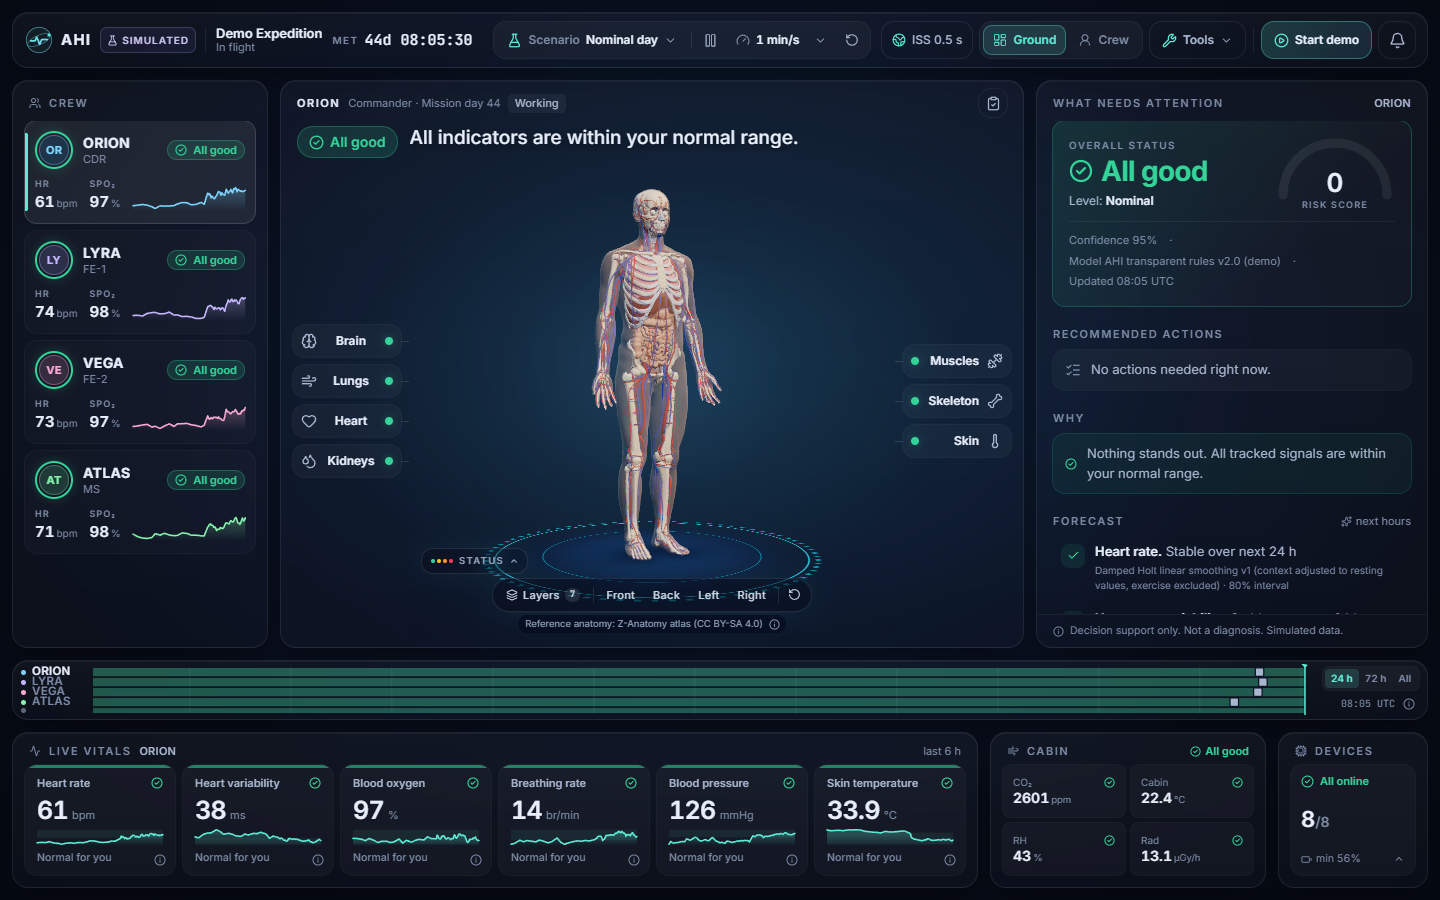
\includegraphics[width=0.54\linewidth]{images/screens/ground-view.png}};
\begin{scope}[x={(img.south east)},y={(img.north west)}]
\node at (0.62,0.955) {\callout{1}};
\node at (0.10,0.60) {\callout{2}};
\node at (0.40,0.62) {\callout{3}};
\node at (0.86,0.60) {\callout{4}};
\node at (0.50,0.23) {\callout{5}};
\node at (0.30,0.12) {\callout{6}};
\end{scope}
\end{tikzpicture}
\captionof{figure}{Ground view on a nominal day, with its six areas numbered. Simulated data.}
\label{fig:ground-view}
\end{minipage}
\par\medskip

\begin{enumerate}
\item[\callout{1}] \textbf{Top bar:} \texttt{SIMULATED} badge, mission profile (Launch, ISS, Moon, Mars transit), mission time, \textbf{scenario player} (scenario, play, speed, restart), \textbf{Earth link}, \textbf{Ground / Crew} toggle, \textbf{Tools}, \textbf{Start demo} and the \textbf{alerts bell}.
\item[\callout{2}] \textbf{Crew rail} (left): one card per astronaut (ORION, LYRA, VEGA, ATLAS) with status in plain words, heart rate, blood oxygen and a six hour sparkline. Click a card or press \key{1} to \key{4}; the rest of the screen follows.
\item[\callout{3}] \textbf{3D body} (center): body systems that need attention light up in their status color; the heart beats at the live heart rate and the lungs breathe at the live breathing rate. Body system chips sit beside it.
\item[\callout{4}] \textbf{What needs attention} (right): status, risk score, actions, reasons and forecast.
\item[\callout{5}] \textbf{Status timeline:} one lane per astronaut plus the cabin, with markers for alerts, actions, check-ins and messages.
\item[\callout{6}] \textbf{Live vitals, cabin and devices} (bottom): six vitals against the personal normal, cabin CO\textsubscript{2}, temperature, humidity and radiation, and the state of every device.
\end{enumerate}


\section{Tutorial: A Mission in Seven Steps}
\label{sec:tutorial}


\subsection{Step 1: Let the guided demo drive}
\label{subsec:guided-demo}

\sidefig{0.68}{Click \textbf{Start demo} in the top bar. A ten step tour spotlights each part of the screen and sets up every scene by itself (\ref{fig:guided-demo}), from the crew and the body to an acute event, slow fatigue, the what-if, the Crew view and the mission tools. Use \textbf{Next} and \textbf{Back} (or \key{$\rightarrow$} and \key{$\leftarrow$}), \textbf{Auto} to advance by itself (about two minutes) and \key{Esc} to leave; leaving restores a calm nominal day. Steps 2 to 7 do the same things by hand.}{images/screens/guided-demo.png}{Guided demo, step 1 of 10: ``Meet the crew''.}{fig:guided-demo}

\subsection{Step 2: Read one astronaut's status}
\label{subsec:read-status}

\sidefig{0.70}{Select ORION in the crew rail. The \textbf{What needs attention} panel (\ref{fig:attention}) answers four questions:
\begin{itemize}\setlength\itemsep{1pt}
\item \textbf{How is he?} The \textbf{overall status}, the \textbf{risk score} from 0 to 100 and the \textbf{confidence}, which falls when key signals are missing (``Status cannot be confirmed'' if core vitals are absent).
\item \textbf{What to do?} \textbf{Recommended actions} with their rationale, priority and an \textbf{autonomy badge}: \textit{Can act on board now}, \textit{Needs flight surgeon}, or \textit{Earth reply in N min+} when Earth is far. \textbf{Mark done} logs the action in the audit trail, \textbf{Dismiss} hides it and \textbf{Compare} opens the what-if (Step 6).
\item \textbf{Why?} Contributing factors in plain words with a weight bar, for example ``HRV 28\% below personal baseline for 3 days''.
\item \textbf{What next?} A forecast per metric, such as ``Projected to leave your normal range in about 5 h''.
\end{itemize}}{images/screens/attention-actions.png}{What needs attention during a critical event.}{fig:attention}

\subsection{Step 3: Explore the 3D body}
\label{subsec:body}

Click the \textbf{Heart} chip beside the body. The camera flies to the heart, the rest of the body becomes a ghost and the right panel shows the \textbf{body system detail} (\ref{fig:body-detail}): each metric with its deviation (``11\% above your normal'') and normal range. Expand a row for the \textbf{trend chart}: the shaded band ``Your normal'', the history (a gap means no data), the dashed \textbf{forecast cone} (80\% interval) and a \textbf{horizon picker} from 24 hours to 15 days. ``Why is this my normal?'' shows the window, median and MAD behind the band.

Click any structure, such as the skull, to see its name and \textbf{Measured by}, the devices that feed it; structures that nothing measures are \textit{Context only}. Drag to rotate, scroll to zoom, and use the pill under the body for \textbf{Layers}, skin opacity and the \textbf{Front, Back, Left, Right} views (\ref{fig:atlas-layers}).

\screenpair{images/screens/body-detail.png}{Body system detail: heart selected, metrics against the personal normal, trend and forecast.}{fig:body-detail}{images/anatomy/atlas-layers.jpg}{Layer presets of the Z-Anatomy atlas \cite{z_anatomy}: default, skeleton, muscles, organs and vessels.}{fig:atlas-layers}

\subsection{Step 4: Respond to a critical alert}
\label{subsec:alert}

\sidefig{0.58}{In the scenario player choose \textbf{Acute cardio event} at \textbf{1 min/s} and press play (\key{Space}). In about seven seconds ORION's heart rate rises at rest while his blood oxygen falls: a red \textbf{critical banner} appears, the bell pulses, a sound rings and the heart and lungs glow through the chest (\ref{fig:critical}).
\begin{enumerate}\setlength\itemsep{1pt}
\item Click \textbf{Mark done} on ``Pause activity, rest, and request flight surgeon review''.
\item Press \key{A}, then \textbf{Acknowledge}: the sound stops. \textbf{View} jumps to the metric.
\item Unacknowledged alerts escalate after 5 and 15 simulated minutes, and a health packet goes to Earth.
\end{enumerate}}{images/screens/critical-alert.png}{Acute cardiac event: critical banner, heart and lungs highlighted, risk score 100.}{fig:critical}

\subsection{Step 5: Spot a slow drift}
\label{subsec:drift}

Choose \textbf{Progressive fatigue} at \textbf{1 h/s} and select LYRA (\key{2}). Over about two simulated days her sleep shortens, her heart rate variability falls below her own band and her resting heart rate drifts up. No single value crosses a line, yet the combined rule moves her to \textit{Keep an eye} and then \textit{Act soon}. Her lane on the \textbf{status timeline} shows the pattern building (\ref{fig:timeline}); choose 24 h, 72 h or All and click a marker to jump to that moment.

\subsection{Step 6: Compare ``what if''}
\label{subsec:whatif}

On LYRA's ``Sleep extension'' action, click \textbf{Compare}. The dialog (\ref{fig:whatif}) projects heart rate variability for 48 hours \textbf{with} and \textbf{without} the action, against her personal normal, lists its assumptions and states: ``Simulation for discussion only. Not evidence of clinical efficacy.''

\screenpair{images/screens/timeline-fatigue.png}{Progressive fatigue: LYRA's timeline lane drifts from green to amber and orange.}{fig:timeline}{images/screens/whatif.png}{What-if: heart rate variability with and without a sleep extension.}{fig:whatif}

\subsection{Step 7: Switch to the Crew view and check in}
\label{subsec:crew-view}

\sidefig{0.58}{Press \key{V}. The \textbf{Crew view} (\ref{fig:crew-view}) is for the astronaut the data is about: a large status word, one sentence, at most two actions (``Do this now'', ``Do this soon'', ``When you can''), cards per body system and ``Your body vs your normal'', with no risk score or model detail.

Click \textbf{Start check-in} for the 30 second daily questionnaire: mood, fatigue, stress and sleep on a 1 to 5 scale, symptom tags and a note. Answers are compared with the person's own history; they support objective signals and never raise an alert alone. Press \key{V} to return.}{images/screens/crew-view.png}{Crew view: status word, top actions, check-in and values against the personal normal.}{fig:crew-view}


\section{Mission Tools}
\label{sec:mission-tools}

These tools deal with the realities of a long mission. Open them from the \textbf{Earth link} control and the \textbf{Tools} menu in the top bar.

\begin{itemize}
\item \textbf{Earth link} (\ref{fig:mars}). Profiles go from the ISS (0.5 s one way) and the Moon (1.3 s) to Mars at its closest (about 4 min) and farthest (about 22 min) \cite{nasa_space_communications_seven_things}. \textbf{Send health packet} and \textbf{Request flight surgeon consult} send messages that stay \textit{In transit} until the simulated clock reaches their arrival. Under Mars profiles, high and critical items also get an on board first step for the crew medical officer.
\item \textbf{Mission overview} (\ref{fig:mission}): radiation dose with a projection, exercise adherence, sleep by week, resting heart rate and HRV, per astronaut or for the whole crew. Budgets are labeled \textit{demo configuration, not official limits}.
\item \textbf{Shift handover} (\ref{fig:handover}): a printable report of the last 24 hours. \textbf{Export FHIR R4 Bundle} downloads a standard JSON bundle with pseudonymized identifiers only; \textbf{Send to ground} queues it on the Earth link.
\item \textbf{Data and model} (\ref{fig:datamodel}): where every number comes from. Real NASA OSDR blood panels from the Inspiration4 mission \cite{osdr_osd569,osdr_osd575} with provenance and file hash, the simulated devices, the model card and the data origin labels. OSDR data is historical reference only and never feeds the alerts.
\end{itemize}

\screenpair{images/screens/mars-comms.png}{Earth link, farthest Mars profile: messages in transit and the on board first step.}{fig:mars}{images/screens/mission-overview.png}{Mission overview: radiation dose, exercise, sleep, resting heart rate and HRV.}{fig:mission}

\screenpair{images/screens/handover-report.png}{Shift handover report with print and FHIR R4 export.}{fig:handover}{images/screens/data-model.png}{Data and model: a real NASA OSDR panel with its provenance.}{fig:datamodel}


\section{Scenario Reference}
\label{sec:scenarios}

Pick a scenario in the scenario player, set the suggested speed (simulated time per real second) and press play. Any scenario runs under any mission profile.

\begin{table}[H]
\centering
\vspace{0.4em}
\caption{The seven scripted scenarios, what to look for and the suggested speed. All simulated.}
\label{tab:scenarios}
\footnotesize
\begin{tabular}{p{2.8cm}p{1.6cm}p{7.6cm}p{1.4cm}}
\hline
\textbf{Scenario} & \textbf{Who} & \textbf{What to look for} & \textbf{Speed} \\
\hline
Nominal day & Everyone & Everything stays green and the risk score is 0. No false alerts. & any \\
Acute cardio event & ORION & Heart rate up at rest, blood oxygen down; critical banner in about 7 s, sound, escalation & 1 min/s \\
Sensor failure & VEGA & The Bio-Monitor shirt goes degraded, stale and offline; organs turn grey and still, the card says \textit{Signal lost} & 1 min/s \\
Cabin CO\textsubscript{2} rise & Cabin & CO\textsubscript{2} climbs; breathing and reaction time shift for everyone; the platform reports co-occurrence, not cause & 10 min/s \\
Progressive fatigue & LYRA & Shorter sleep, lower HRV, higher resting heart rate over days; \textit{Keep an eye}, then \textit{Act soon} & 1 h/s \\
Exercise decline & ATLAS & Workout output falls day after day; the muscles layer appears & 1 h/s \\
Eye changes (SANS like) & ORION & Click the Eyes chip: eye exam history against the preflight baseline, per eye & any \\
\hline
\end{tabular}
\vspace{0.6em}
\end{table}

\sidefig{0.70}{Slow scenarios stop at \textit{Act soon}: they call for review, not an emergency. Only the acute cardio event reaches \textit{Act now}.

The sensor failure is a data quality case: the organs fed by the failed device turn grey and still and are labeled no data, so a lost signal never looks normal (\ref{fig:atlas-states}).}{images/anatomy/atlas-states.jpg}{Status on the body: (a) acute cardiac event; (b) sensor failure, every region grey and labeled no data.}{fig:atlas-states}


\section{Accessibility, Languages and the Assistant}
\label{sec:access}

AHI says important things in more than one way (settings in \textbf{Tools > Accessibility and sound}).

\begin{itemize}
\item \textbf{Alert sounds:} critical alerts ring every 30 s until acknowledged, and more urgently after 2 minutes.
\item \textbf{Audio description:} \key{D} describes the screen aloud; \key{Shift}+\key{D} keeps speaking new alerts, status changes and selections. Missing data is spoken as ``no data''.
\item \textbf{Keyboard and 3D body:} \key{Tab} reaches the body navigator; arrows move between body systems and structures, \key{Enter} selects. The interface follows WCAG 2.1 practices \cite{w3c_wcag21}.
\item \textbf{Languages:} English by default; Portuguese, Spanish, Japanese and German in \textbf{Tools > Language} (machine assisted, pending native review). \key{P} turns on presentation mode.
\item \textbf{Ask AHI} (bottom right): ask ``How is ORION doing?'' by text or voice. Answers stream, can be read aloud and end with ``Based on:'' naming the data used. The assistant explains engine results and never diagnoses or changes a status. The demonstrator uses the Claude API \cite{anthropic_claude_api}; a mission would use a local model on board.
\end{itemize}

\begin{table}[H]
\centering
\caption{Keyboard shortcuts. Press \texttt{?} in the application to see them all.}
\label{tab:shortcuts}
\small
\begin{tabular}{p{1.8cm}p{3.6cm}p{1.4cm}p{3.6cm}p{1.2cm}p{3.6cm}}
\hline
\textbf{Key} & \textbf{Action} & \textbf{Key} & \textbf{Action} & \textbf{Key} & \textbf{Action} \\
\hline
\key{1} to \key{4} & Select crew member & \key{V} & Ground or Crew view & \key{A} & Open or close alerts \\
\key{Space} & Play or pause & \key{Esc} & Close a panel, go back & \key{D} & Describe the screen \\
\key{P} & Presentation mode & \key{?} & Show all shortcuts & & \\
\hline
\end{tabular}
\end{table}


\section{Troubleshooting and Responsible Use}
\label{sec:troubleshooting}

\textbf{Nothing changes:} press \key{Space} to play (in the nominal day nothing should happen) or use \textbf{Restart}. \textbf{``Reference atlas unavailable'':} a simpler body is shown and everything else works; run \texttt{npm run anatomy:validate}. \textbf{No body at all:} turn on hardware acceleration and reload. \textbf{``Offline demo mode'' with the backend running:} check \texttt{http://localhost:8000/api/v1/health}. \textbf{No sound:} click once in the page.

\noindent\textbf{Responsible use.} When you present AHI, say it with every claim: \textit{the data is simulated, and the tool supports decisions and does not make them}. High and critical items always need human review, and fixed thresholds are demo configuration, not official limits.


\printbibliography

\end{document}
% End of Document %%%%%%%%%%%%%%%%%%%%%%%%%%%%%%%%%%%%%%%%%%%%%%%%%%%%%%
